\documentclass[12pt]{article}

%\usepackage{times} %for Times New Roman, if required
\usepackage[top=1in, bottom=1in, left=1in, right=1in]{geometry} %adjust margins. TODO: hack to fix large top margin
\usepackage{setspace} %allows doublespacing, onehalfspacing, singlespacing
\usepackage{enumitem} %for continuing lists
\usepackage{titling} %for moving the title
\usepackage[normalem]{ulem} %for underlining
\usepackage{graphicx}
\graphicspath{{images/}}

\begin{document}

\begin{spacing}{.4}
\setlength{\droptitle}{-7em}
\title{Genie: A Population Genetics Simulation Built with JavaScript}
\author{Ben Roos}
\maketitle
\newpage
\end{spacing}

\begin{spacing}{1.5}

\section*{Table of Contents}
\begin{enumerate}
\item Introduction
\item Model
\item Implementation
\item Lesson Plan
\item Discussion

\end{enumerate}
\newpage

\section{Introduction}

Web development technologies, and in particular the programming language JavaScript, present a unique opportunity for creating computationally complex educational tools. In many educational settings, it may be useful to develop a tool that allows instructors to demonstrate concepts visually or that allows students to investigate a concept naturally. However, when dealing with certain fields of study, such tools would need to conduct computational simulations. One such field is biology, in which concepts from population genetics and evolution may benefit from programmed stochastic simulations in order to demonstrate certain concepts, such as genetic drift and gene flow, in real time. Given ongoing improvements to modern web browsers and development technologies, programmers can now develop web applications that demonstrate computationally intensive simulations as they run. A web application was developed to demonstrate several concepts from population genetics and evolution, including genetic drift, gene flow, founder effects, and mutations. This application conducts a real time simulation of the change in allele frequencies in a finite population of spatially isolated individuals. Using colors, the application allows students to visualize changes in a population over time and understand how those visual changes translate to fluctuations in allele frequency and, eventually, allele fixation.

\section{Model}

\subsection{Population}
The simulation uses a Moran Model \cite{moran} to describe a finite population of 1024 haploid individuals. The simulation tracks a single allele for each individual. This allele is selected independently for each individual, and the simulation uses an infinite alleles model \cite{moran}, so the alleles are represented using numbers that begin at 0 and may be infinitely high. Each individual is geographically isolated from others in a grid that is 32 cells long and 32 cells wide. Each individual takes up only one cell, and each cell contains only one individual. Thus, the size of the population will never vary from 1024 at any step of simulation.

\subsection{Initializing the Population}
When the simulation initializes, a population is randomly generated. The allele number for each individual in the population is selected sequentially, beginning with the upper left corner of the grid, proceeding through each row from left to right, and ending with lower right corner of the grid. The first individual is immediately assigned the allele number 0. With probability $\displaystyle \frac {i}{i + \theta}$, where i is the number of individuals in the population generated so far, and $\theta$ = 2N$\mu$, where N is the number of individuals in the population and $\mu$ is the mutation rate, subsequent individuals in the population will be an assigned an allele number equal to that of a randomly selected member of the population. With probability $\displaystyle 1 - \frac{i}{i + \theta}$, subsequent individuals are assigned to new allele numbers, momentarily becoming the only member of the population with the given allele. Thus, individuals that are assigned alleles earlier in the initialization process are more likely to be assigned new alleles, while individuals that are assigned later in the process are more likely to be assigned an allele from the population.

\subsection{Simulation}
At each step of the simulation, a randomly selected individual dies, leaving its corresponding cell momentarily empty. A parent allele is then randomly selected from the immediate neighbors of the empty cell. Each cell's neighbors include the eight cells that are either immediately adjacent to or diagonal from the cell. This simulation also has edge effects because empty cells on the edges or corners of the grid will have fewer neighbors than other cells. With probability 1 - $\mu$, the new individual will have the same allele as its parent, and with probability $\mu$ a mutation will occur, and a unique allele number will be assigned to the new individual. 2000 steps occur during each ``generation," and the population is redrawn in the visualization once for each generation.

\section{Implementation}

\subsection{Design}

\subsubsection{Layout}
The application contains three components: a control panel, with which users can control the simulation and its parameters; a grid, on which the simulation is displayed; and graphs, on which statistics regarding the simulation are shown. The layout of the application is shown in Figure 1.
\begin{figure}[h]
\caption{Layout of Genie on Page Load}
\centering
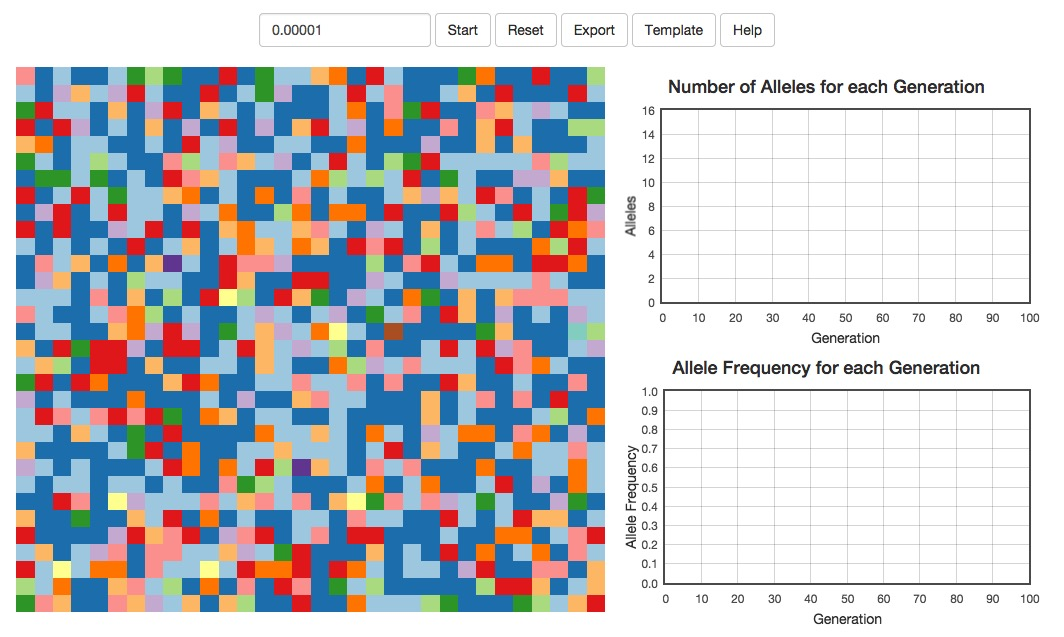
\includegraphics[scale=0.4]{layout}
\end{figure}

\subsubsection{Input Paremeters}
The control panel includes a text field in which users can enter the mutation rate that will be used during the simulation. The default mutation rate is 0.00001, and is displayed in the text field when the page loads.

\subsubsection{Running the Simulation}
To start and pause the simulation, users click on a single button, which will display either ``Start" or ``Pause" depending on whether the simulation is running. Users can reset the simulation by clicking ``Reset." This control generates a new initial population, reinitializes the grid, and clears the graphs.

\subsubsection{Barriers}
Users also have the ability to create a barrier in a cell by clicking on the desired cell. When a barrier is created, the allele number is set to -1 and color associated with the cell is \#000000 (black). Barriers cannot act as parent cells, so they are never replicated, and barriers cannot die during the simulation and subsequently be replaced. Thus, using barriers, users can construct physical constraints around which the movement of alleles of subpopulations is restricted. Users can create multiple barriers by clicking on multiple cells or by clicking and dragging. If users want to remove a barrier, they can click on the chosen cell a second time. This action will set its allele number to -2 and its color to \#FFFFFF (white). In this state, the cell can be considered empty; neighboring cells can replicate their alleles into an empty cell, but it cannot be chosen as a parent. Barriers can be cleared either by clicking or by clacking and dragging.

\subsubsection{Barrier Templates}
If users are running a local copy of the application, they can also create templates of barriers so that barrier patterns can be applied with a single click. In order to create a template, users must first create the barrier pattern that they would like to save by clicking, or clicking and dragging, over the cells that should be barriers. Users can then export the grid to a JSON object by clicking ``Export." They can then locate BarrierTemplate.js in their local copy of the application. They should replace the JSON object that is assigned to the barrierTemplate variable with the JSON object that they just downloaded. Now, in their local copy, the ``Template" button on the control panel will refer to the barrier pattern they defined.

\subsubsection{Forced Mutations}
Users can force a mutation to occur in a similar manner to creating barriers. By holding the SHIFT button while clicking, or clicking and dragging, they can force grid cells to contain individuals with mutant alleles. When a user performs this action, the allele number is changed to the mutant allele number and a new color is assigned to the cell.

\subsubsection{Export}
If users would like to export a JSON representation of the population at a given point in the simulation, they can click ``Export" while the simulation is paused. The format of the JSON object is \ \texttt{\{cells:[\{color:hex\_val,allele:[-2,$\infty$),mutationNumber:[0,$\infty$\},\{...\},...] \}}. Each cell object includes the CSS hex value for the color associated with the allele, the allele number, and the mutation number, and the JSON object that is created is a list of these cell objects. The allele number varies from -2 to $\infty$ because the allele number -1 refers to cells occupied by a barrier and -2 refers to cells that are unoccupied. All other allele numbers are identifiers of a unique allele.

\subsubsection{Graphs}
Two graphs are displayed to the right of the grid. The upper graph displays the number of unique alleles in the population over time and the lower graph displayed the allele frequencies of each unique allele in the population over time. In the lower graph, the colors associated with each allele match the colors of the simulation. Both of these graphs update in real time as the simulation is running.

\subsection{Architecture}
The simulation was written entirely in JavaScript \cite{jsTutorial}, using jQuery \cite{jQuery}, Bootstrap \cite{bootstrap}, HTML \cite{htmlTutorial} and Cascading Style Sheets (CSS) \cite{cssTutorial}. In order to logically structure the code, the application was built using the revealing module design pattern \cite{js}. Using this design pattern, each module refers to a distinct portion of the application, and enables each module to contain public and private methods. Similar to a singleton pattern, the revealing module pattern creates a single instance of each JavaScript object. To organize this application's source code, one module was created for each major component: the control panel, the grid, and the two plots. A cell object was also defined to keep track of the allele number and color of each individual in the population. This object was defined using the constructor pattern \cite{js} rather than the module pattern so that many cells could be declared. Unlike the other objects, cell does not act as a singleton, and 1024 instances of cell are created to correspond to each individual.

\subsubsection{Control Panel}
The control panel refers to the series of buttons and text field above the grid. This method only contains event handlers for each of the buttons and the text field included in the control panel. Thus, it contains an event handler for the ``Start," ``Stop," ``Reset," ``Export," ``Template," and ``Help" buttons. With the exception of the ``Help" button, each of these buttons simply invokes behavior from the Grid module, in addition to conducting basic error handling to ensure that a nonnegative, nonempty value has been entered for the mutation rate. As a result, each event handler simply calls functions defined in that module. The ``Help" button is a simple link to the README hosted on GitHub at the URL github.com/benhroos/thesis. The structure of this module is shown in Figure 2.
\begin{figure}[h]
\caption{Class Diagram for Control Panel Module}
\centering
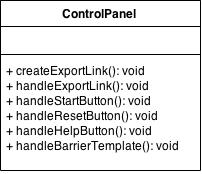
\includegraphics[scale=0.5]{control-panel-class-diagram}
\end{figure}

\subsubsection{Grid}
The grid refers to the visual representation of the population by the web application. The grid is 32 cells wide and 32 cells long, and is the primary visualization tool of the application. The logic that drives the grid is encapsulated in a JavaScript module in a file named grid.js.\newline
\newline
This module includes two methods to generate colors to represent each allele. getColor() generates selects a CSS hex value from an array of predetermined hex values each time a new allele is generated in the founding population, and getMutantColor() generates a CSS hex value from a separate array of predetermined hex values each a time a mutant allele is generated over the course of the simulation. The 18 colors in the first array were chosen from ColorBrewer such that they would appear distinct beside each other. Only 18 colors were used because, in the initial population, the number of unique alleles is almost always less than 18 (and, even if the number was initially greater than or equal to 18, it would very quickly decrease), and the distinctness of the colors was weighed more heavily than the uniqueness. The 6 colors in the array of mutant colors were selected for their brightness, to distinguish them from alleles in the founding population. Only 6 colors were used because, for a realistic mutation rate, very few mutant alleles consistently thrive in the model.\newline
\newline
This module also contains a method to perform one step of the simulation. Recall that, when a step occurs, a random individual dies. With probability $\mu$, a mutant allele is created, and with probability $1 - \mu$, a parent cell is randomly chosen from one of the cell's immediate neighbors. It also contains a method to run the simulation for 1 ``generation," or 2000 steps.\newline
\newline
The module contains a method to redraw the grid on the web page. This is done using a setInterval() method, such that the grid is redrawn every 200 milliseconds, and 1 generation has passed each time the grid is drawn. This method also updates the graphs that show the number of alleles and the allele frequencies.\newline
\newline
The module contains a couple of methods to handle actions that can be performed on the grid. One method is used to create barriers, and uses jQuery event handlers to detect when a user has clicked, or clicked and dragged, on particular cells and behaves accordingly. It contains a very similar method to handle forced mutations.\newline
\newline
Finally, the module contains a method to initialize the grid by selecting the founding population in the manner previously described. The structure of this module is shown in Figure 3.
\begin{figure}[h]
\caption{Class Diagram for Grid Module}
\centering
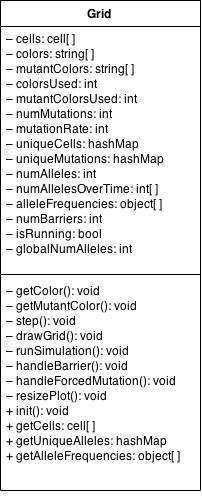
\includegraphics[scale=0.5]{grid-class-diagram}
\end{figure}

\subsubsection{Plots}
There are two modules to control the graphs: one for the graph showing number of alleles and one showing the graph for the allele frequencies. Each module is very similar, and contains a method to initialize the plot when the web page is first loaded and a method to update the plot with new data. The latter method simply redraws the plot with updated axes, updated data, and the ability to pan through the graph. For these graphs, the plotting library flot \cite{flot} was used. flot was chosen for the number of graph options and plugins that were available, and for ease of use based on previous familiarity. However, several other plotting libraries would provide similar functionality for the purposes of this web application. The structure of these modules is shown in Figure 4.
\begin{figure}[h]
\caption{Class Diagram for Control Panel Module}
\centering
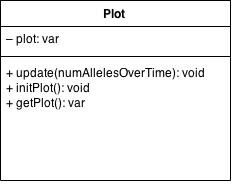
\includegraphics[scale=0.5]{plot-class-diagram}
\end{figure}

\subsubsection{Cell}
The cell object has attributes to store the color and allele number of each individual, as well as whether a mutation has occurred. It has an attribute, mutationNumber, that is -1 if a mutation has not occurred for that cell, and is otherwise equal to the number of mutations that had occurred when a mutation occurred for that cell. These attributes are stored in a constructor to instantiate each cell with an allele number. The only method in the object is updateHTML(), which updates the background color of a grid cell when the allele number changes. The structure of this object is shown in Figure 5.
\begin{figure}[h]
\caption{Class Diagram for Control Panel Module}
\centering
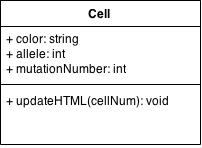
\includegraphics[scale=0.5]{cell-class-diagram}
\end{figure}

\subsubsection{Sequence of Interactions}
In a typical sequence of interactions using Genie, the page would first be loaded, which would trigger a call to Grid.init(), which creates 1024 cell objects and stores then in an array that tracks the entire population throughout the simulation. When a user clicks the ``Start" button, the interval timer that powers to simulation begins to run, conducting 2000 steps of the simulation, drawing the grid every 200 milliseconds, and updating the plots. When the user clicks ``Stop," the interval will be cleared and the timer will stop. If the user clicks any combination of the buttons in the control panel, it will simply trigger the event callback defined in the Control Panel module. A sequence diagram demonstrating a typical interaction is shown in Figure 6.
\begin{figure}[h]
\caption{Class Diagram for Control Panel Module}
\centering
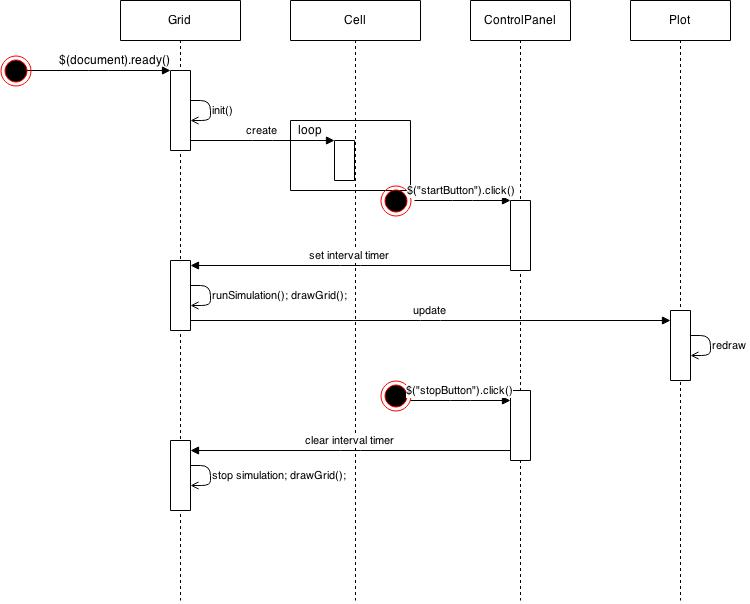
\includegraphics[scale=0.5]{sequence-diagram}
\end{figure}

\section{Lesson Plan}

As mentioned previously, this application may be particularly useful for educational uses. Because the application can be run in any modern web browser, on any platform, students should easily be able to access the application and use it to improve their understanding of several concepts from genetics and evolution classes, including genetic drift, founder effect, gene flow, and speciation. Following is a description of some of these concepts.\newline
\newline
Genetic drift is the variation of allele frequencies in a population from one generation to the next that is attributed to variation from random sampling \cite{evolution}. When a small sample is taken from a larger population, the sample is not likely to contain the same allele frequencies, or the same number of unique alleles, that were represented in the larger population. Essentially, it is unlikely that the small sample is representative of the larger population. Genetic drift has the potential to affect all populations, but its effects are especially noteworthy in small population, in which variation caused by sampling is more likely to occur. These variations from sampling can cause the allele frequencies to fluctuate from one generation to the next, particularly in small populations \cite{evolution}. Because the allelic composition of each generation forms the starting point for the subsequent generation, these random variations in each generation can propagate to significant fluctuations in the allele frequencies of a population over time. Given enough generations, one allele will eventually reach fixation in the population, simply due to random chance, even when no element of fitness is present \cite{evolution}. This simulation is particularly suited to demonstrate this phenomenon because the model does not contain any element of fitness. All variations in allele frequency that are observed in the simulation are simply caused by random sampling.\newline
\newline
Founder effects are strongly related to genetic drift. When a small subpopulation forms a new population, the allele frequencies in the new founding population may not be representative of the larger population. This is simply caused by random sampling, much like genetic drift. Because the founding population is not likely to have the same allele frequencies as the larger population, the subsequent population is likely to have a genetic makeup that differs from the population from which it was sampled \cite{genAnalysis}.\newline
\newline
Gene flow is the migration of individuals between populations. When migrating individuals reproduce in their new population, the result is a mixed population, with alleles from both populations playing a role in determining the genetic makeup of the subsequent population. Gene flow, much like genetic drift, has the potential to change the frequency of alleles in the new, mixed population \cite{genAnalysis}. If two populations start with radically different allele frequencies, the subsequent mixed population will likely have different allele frequencies from either starting population, quickly causing evolutionary change in the populations. Additionally, gene flow can have an equalizing or homogenizing effect on the allele frequencies of the populations involved, causing an overall loss of genetic diversity \cite{genAnalysis}.\newline
\newline
After explaining the model used by the simulation, students should answer the following questions. Each question is preceded by a learning objective in bold and is followed by a sample answer in italics.

\subsection{Genetic Drift}
\begin{enumerate}
\item
\par \textbf{Learning objective: students with think critically about why some populations are susceptible to the effects of genetic drift.}
\par The population represented in this simulation consists of only 1024 individuals, and the population does not expand as the simulation is run. Do you expect that genetic drift will have a significant effect on this population? Explain your answer. Run the simulation for approximately 100 generations. Has genetic drift occurred? How does this result compare with your answer to the previous question?
\par \textit{Genetic drift is caused by errors in sampling. We would only expect these errors to have a significant effect on allele frequencies in the population if only a small number of individuals are producing the next generation. Because the population in this simulation is small, we would expect genetic drift to have a significant effect.}
\item
\par \textbf{Learning objective: students will think critically about the impact of genetic drift.}
\par If you allow the simulation to run indefinitely, what effect would you expect on allele frequencies in the long term? Allow the simulation to run for 300 generations. What effect does this have on allele frequencies? How does this result compare with your answer to the previous question?
\par \textit{Over many generations, random genetic drift will eventually lead to allele fixation. We would expect that if the simulation is run indefinitely, the population would eventually reach a point of homogeneity, in which one allele represents the entire population.}
\item
\par \textbf{Learning objective: students will consider the formation of a new founding subpopulation.}
\par Using the population from the previous step, create a subpopulation in one corner of the grid (recall, you can create barriers by clicking, or by clicking and dragging, on any cell). Can you think of a physical event that would create a subpopulation like this?
\par \textit{Earthquakes, fires, and other natural disasters could cause sudden separation of populations. Over the long term, gradual tectonic shifts may cause a subpopulation to emerge.}
\item
\par \textbf{Learning objective: students will consider founder effects in a subpopulation.}
\par Would you expect the allele frequencies in this subpopulation to differ from the entire population? Using a rough visual estimate, do the allele frequencies of the subpopulation match the allele frequencies of the entire population?
\par \textit{There is a high likelihood that they allele frequencies do not match, and that the subpopulation has less genetic diversity than the larger population.}
\item
\par \textbf{Learning objective: students will identify founder effects.}
\par What caused the difference in allele frequencies between the sample population and the population as a whole? Compare this phenomenon to the effect of genetic drift.
\par \textit{The subpopulation is made up of very few individuals, and is drawn from an already small population. As a result, the differences in allele frequency are simply due to random variation from sampling. This has a very similar effect to genetic drift, and if this subpopulation continues to be isolated from the larger population, the difference in allele frequencies is called the founder effect. The population that results from this subpopulation may have drastically different allele frequencies to the original population}
\item
\par \textbf{Learning objective: students will identify the future impact of founder effects.}
\par If the simulation is run for several more generations, what effect would you expect to occur on the genetic diversity of the subpopulation? Run the simulation for several more generations and compare the results with your prediction.
\par \textit{This population has suffered a loss of genetic diversity from the gene pool of the whole population. We would expect allele fixation to occur more rapidly in this subpopulation}
\item
\par \textbf{Learning objective: students will use practice knowledge from previous exercises to predict the impact of genetic drift.}
\par Reset the grid to create a new founding population. Then apply the default template (by pressing the ``Template" button). This should create four spatially isolated subpopulations. What do you expect to happen to the allele frequencies of these subpopulations when you run the simulation? Would do you expect to happen to the allele frequencies of the entire population? Run the simulation for 200 generations and compare the results to your predications.
\par \textit{We would expect the four subpopulations to reach allele fixation quickly, but it is likely that each subpopulation will be represented by a different allele. Thus, the population as a whole would have 4 equally prevalent alleles.}
\end{enumerate}

\subsection{Gene Flow}
\begin{enumerate}
\item
\par \textbf{Learning objective: students will visualize the impact of isolation by distance.}
\par Using the population created in the previous question, run the simulation until allele fixation occurs for every subpopulation. How many generations did this take? Do you expect that this number is the same for every simulation?
\par \textit{This typically takes around 200 ``generations," but results vary. This may warrant discussion on why results differed for some students. Because the simulation (and the phenomenon has an element of randomness, we do not expect results to match every time.}
\item
\par \textbf{Learning objective: students will predict the impact of gene flow on discrete populations.}
\par Remove all barriers between the left and right subpopulations, such that there is still a barrier dividing the population horizontally, but not vertically. What do you expect to happen to the allele frequencies of the subpopulations?
\par \textit{We expect that the allele frequencies in these new subpopulations will fluctuate, and that allele fixation will eventually occur again.}
\item
\par \textbf{Learning objective: students will predict the effect of limited migration between populations}
\par Create a path for migration between the 2 subpopulations by removing 2 of the barriers between them (the path should be 1 cell wide). What do you expect to happen to the allele frequency of the subpopulations? Run the simulation for 100 generations and compare the results with your predications.
\par \textit{Some genetic diversity will be introduced to each subpopulation, but because migration is so restricted, it is likely that each subpopulation won't be as quickly impacted as before.}
\item
\par \textbf{Learning objective: students will practice knowledge from previous exercises to predict the effect of gene flow over time.}
\par Remove all barriers from the grid. What do you expect to happen to each subpopulation? What do you expect to happen to the population as a whole?
\par \textit{Allele frequency of the larger population will fluctuate and will eventually reach allele fixation.}
\end{enumerate}

\section{Discussion}

\subsection{Technical Challenges}
During the development of Genie, the most common technical challenge that occurred was optimizing performance for web browsers. While the simulation itself was able to run very quickly in the browser, the visualization needed to be handled separately in order to update in real time. While the simulation itself could be run in a web browser continuously, the browser was not capable of updating the screen output at the same speed. As a result, if the simulation was run continuously, the visualization would simply never update, giving the impression that the simulation was not running at all. In order to give the impression that the simulation was, in fact, updating frequently, the simulation was run in portions based on an interval timer that was set to update every 200 milliseconds. During that interval, 2000 times steps, or one ``generation" of the simulation would be run, then a method would be called to update the user interface with the generational changes, then the plots on the side of the web page would be updated, and the interval would subsequently repeat. Breaking up the simulation into sections of running, updating the interface, and repeating, allowed the browser time to update in real time, giving users the impression that the grid they could see on their screen was representative of the simulation at any given point in time.\newline
\newline
Another substantial challenge was optimizing performance across many browsers and platforms. For the sake of convenience, most testing that was conducted during the primary development phase was performed in Safari, in which performance appeared to be nearly optimal. However, testing in other browsers, including Chrome and Firefox for Mac, Windows, and Ubuntu, quickly revealed that the visualization appeared to update far more slowly, perhaps every half second rather than every fifth of a second, despite the fact that the simulation itself was running at the same speed. Because the simulation clearly was not the source of the reduction in performance, testing revolved around the functions that were responsible for updating the interface. It was discovered that the cause of the reduction in performance was the use of classes as identifiers for jQuery functions. When classes were used, it appeared that the browser faced a performance penalty for retrieving all members of the class at one time. Because this performance penalty was not observed in Safari, it is possible that the browser cached HTML elements for future use in a way that Chrome and Firefox did not. Refactoring these functions to select elements by id, rather than by class, quickly resolved the performance issues and led to improved performance across platforms.

\subsection{Future Improvements}
If development on Genie continues, there are a number of improvements that could be made. In order to give instructors more flexibility in demonstrations of various concepts, it may be useful to provide the ability to use multiple barrier templates, such that a different template could be used to demonstrate different concepts. For example, a user who had a local copy of the simulation running could add a template to demonstrate gene flow and a separate template to demonstrate speciation. These two templates could be named in a JSON formatted template object, and those names could be displayed in unique buttons for each template.\newline
\newline
Another simple improvement would be the addition of a color blind safe mode, which would alternate the color scheme such that color blind students would be able to use and understand the application without issue. While this feature is less crucial to the overall usability of the application, it is a relevant improvement given the setting in which the application would be used. If used in a college lecture with hundreds of students, of which a significant portion are male, it could be assumed that potentially dozens of students would have some form of color blindness, making the application less usable for a significant portion of the class \cite{colorblind}. A color blind safe mode would eliminate this concern for those students.

\subsection{Comparison to Other Tools}
Several other tools currently exist for the purpose of educational instruction in biology. These tools differ greatly in terms of the development technologies used and in terms of usefulness. Genie represents an attempt to develop a unique tool that provides an alternate use case to previously developed tools. One tool that bears some similarities to Genie is RedLynx \cite{redlynx}, a population genetics simulator similarly built using JavaScript. Because RedLynx was developed using JavaScript, and because all computations are subsequently performed on the client, RedLynx is similarly well-suited for use by instructors during lectures and assignments. This implementation allows students to run the simulator in the convenience of a web browser, from any internet-connected computer. RedLynx also similarly tracks the frequency of an allele in a population over many generations, and provide many input parameters that Genie does not use, including the population size, the frequency of the allele, the number of generations, and parameters pertaining to selection \cite{redlynx}. Although Genie does not allow for the customizability that RedLynx provides, Genie has the unique advantage of running the simulation in real time, allowing students to not only visualize the results of the simulation, but to actually watch the simulation as it runs. This visualization tool helps students understand the fluctuations of allele frequencies in a unique way because they can actually watch the fluctuation of allele frequencies.\newline
\newline
Another tool for visualizing and simulating genetic processes is Populus \cite{populus}. Populus, like RedLynx, provides far greater flexibility than Genie. This flexibility extends not only to the input parameters that can be specified, but also to the types of simulations that can be run. For an instructor looking for a more expansive tool, Populus may be a better choice. However, because of the enormous number of options available, Populus may be more well-suited to be used by instructors during demonstrations than by students during assignments. Unless students thoroughly familiarized themselves with the software before beginning, it is possible that an assignment would require a step-by-step tutorial in order to use the software effectively. Additionally, because Populus is implemented in Java as a .jar file, students would need to have Java installed prior to use. Because Genie can be run in any modern web browser, the vast majority of students will be able to use Genie without any additional preinstalled software.\newline
\newline
The Darwin project at the University of Connecticut is similarly implemented in Java \cite{uconn}. However, through the use of Java applets, the simulations are similarly able to be viewed in a web browser. However, despite this ability, Java still needs to be installed on users computers in order for the simulation to run, giving the same limitations described above. Additionally, many browsers now block Java applets from running for security purposes, and the home page for the tool contains a note that ``Recent updates to Java mean that the applets only work if you disable Java security \cite{uconn}." This limitation demonstrates many of the advantages of a JavaScript implementation. While Java updates can sometimes lead to issues of incompatibility, JavaScript is the primarily programming language of web, meaning that JavaScript code is likely to be supported by browsers for many years, reducing the overall maintenance cost of Genie's implementation.

\subsection{Conclusion}
Genie provides a unique tool to allow instructors to demonstrate concepts, including genetic drift, founder effect, and gene flow, to a large group of students. Additionally, Genie's implementation in JavaScript allows it to be run from virtually any modern computer, giving students the ability to use the tool on their own, to either explore the concepts naturally or to complete assignments. Additionally, because the tool provides few options for students to adjust input parameters, assignments need not include lengthy tutorials or instructions that students need to follow. The primary focus of the tool is visualization in order to improve understanding. By drawing the population in a user's browser while the simulation is ongoing, Genie may allows students to gain a more natural grasp on concepts in population genetics and evolution.

\begin{thebibliography}{9}

\bibitem{bootstrap}
Bootstrap: The world's most popular mobile-first and responsive front-end framework. (2015). Retrieved from http://getbootstrap.com

\bibitem{redlynx}
Cartwright, R. (2012, January 1). Red Lynx: Population Genetics Simulator. Retrieved from http://scit.us/redlynx/

\bibitem{cssTutorial}
CSS Tutorial. (2015). Retrieved from http://www.w3schools.com/css/

\bibitem{moran}
Ewens, W. (1979). Infinitely Many Alleles Model. In \textit{Mathematical Population Genetics} (2nd ed.). New York City, New York: Springer-Verlag.

\bibitem{colorblind}
Facts About Color Blindness. (2015, February 1). Retrieved from https://www.nei.nih.gov/health/color\_blindness/facts\_about

\bibitem{uconn}
Holsinger, K. (1999, September 20). Population Biology Simulations. Retrieved from http://darwin.eeb.uconn.edu/simulations/simulations.html

\bibitem{htmlTutorial}
HTML(5) Tutorial. (2015). Retrieved from http://www.w3schools.com/html/

\bibitem{jsTutorial}
JavaScript Tutorial. (2015). Retrieved from http://www.w3schools.com/js/

\bibitem{jQuery}
JQuery. (2015). Retrieved from http://jquery.com. The jQuery Foundation.

\bibitem{js}
Osmani, A. (2012). JavaScript Design Patterns. In \textit{Learning JavaScript Design Patterns} (Vol. 1.6.1). Sebastopol, CA: O'Reilly Media.

\bibitem{populus}
Populus. (2015, March 19). Retrieved from http://www.cbs.umn.edu/research/resources/populus

\bibitem{genAnalysis}
Sanders, M., \& Bowman, J. (2012). Population Genetics and Evolution. In \textit{Genetic Analysis: An Integrated Approach} (pp. 751-753, 758-760). Benjamin Cummings.

\bibitem{flot}
Schnur, D. (2014). Attractive JavaScript plotting for jQuery. Retrieved from http://www.flotcharts.org

\bibitem{evolution}
Zimmer, C., \& Emlen, D. (2013. The Ways of Change. In \textit{Evolution: Making Sense of Life} (pp. 159-165). Greenwood Village, Colorado: Roberts and Company.

\end{thebibliography}

\end{spacing}
\end{document}

